\documentclass{article}
\usepackage{graphicx} % Required for inserting images
\usepackage[a4paper, left=2.00cm, right=2.00cm, bottom=2.00cm, top=2.00cm]{geometry}
%\usepackage[a4paper, total={6.5in, 9.5in}]{geometry}
\usepackage{authblk}
\usepackage[T1]{fontenc}
\usepackage{palatino}
\usepackage{enumitem}
\usepackage{tikz} %bikin grid
\usepackage{amsmath} %bikin matriks
\usepackage{tabularray} %bikin matriks
\UseTblrLibrary{amsmath} %bikinmatriks
\usepackage{authblk}
\usepackage{listings}
\usepackage{color}
\usepackage{hyperref}
\usepackage{booktabs} 

\definecolor{dkgreen}{rgb}{0,0.6,0}
\definecolor{gray}{rgb}{0.5,0.5,0.5}
\definecolor{mauve}{rgb}{0.58,0,0.82}
\definecolor{dkred}{rgb}{0.8,0,0}

\lstset{frame=tb,
  language=Matlab,
  aboveskip=3mm,
  belowskip=3mm,
  showstringspaces=false,
  columns=flexible,
  basicstyle={\ttfamily},
  numbers=none,
  numberstyle=\small \ttfamily \color{dkred},
  keywordstyle=\color{blue},
  commentstyle=\color{dkgreen},
  stringstyle=\color{mauve},
  breaklines=true,
  breakatwhitespace=true,
  tabsize=3
}

\renewcommand\thesection{\arabic{section}.}
\renewcommand\thesubsection{\alph{subsection}.}
\renewcommand*\figurename{Gambar}
\renewcommand*\tablename{Tabel}
\renewcommand*\lstlistingname{Source code}

\title{\textbf{Tugas 4 Metode Inversi}}
\author{\textbf{Jasinda Wijdannysa (5001201147)}}
\affil{Departemen Fisika, Institut Teknologi Sepuluh Nopember}
\date{}

\begin{document}

\maketitle

\section*{Link Video Penjelasan}
Berikut ini merupakan \textit{link} penjelasan jawaban dari soal di bawah.\\
\href{https://youtu.be/KvT1jMEQwBE}{\textbf{\underline{https://youtu.be/KvT1jMEQwBE}}}


\section{Jelaskan keuntungan dan kelebihan dari optimasi global dibandingkan dengan optimasi lokal!}
Optimasi global umumnya lebih mudah digunakan untuk mencari solusi yang paling baik dibandingkan dengan optimasi lokal.
Pada optimasi global, pencarian dapat dilakukan secara berurutan ataupun secara acak untuk mendapatkan solusi global minimum yang paling baik.
Optimasi global, berfokus untuk mencari solusi terbaik, maka diperlukan iterasi yang banyak dan waktu yang cukup lama dibandingkan dengan optimasi lokal untuk menemukan solusi minimumnya.
Optimasi global juga lebih kompleks dibandingkan dengan optimasi lokal, di mana optimasi global hanya akan mencari solusi yang paling baik diantara banyaknya lokal minimum, atau bisa dikatakan solusi yang paling minimum.
Kelebihan lain dari optimasi global adalah, tidak diperlukannya turunan jacobian atau pemodelan kedepan yang digunakan sebagai model awal untuk dapat mencari solusinya.
Lalu, optimasi global dapat digunakan untuk pencarian solusi pada fungsi yang memiliki parameter-parameter yang sangat banyak atau kompleks.
Jika dibandingkan dengan optimasi lokal, optimasi lokal hanya lebih mudah digunakan untuk permasalahan atau fungsi dengan parameter sederhana, namun ketika diberikan fungsi kompleks, maka optimasi lokal sudah tidak akurat lagi untuk digunakan.


\bigskip
\section{Jika data digenerasi ($d_{obs}$) menggunakan persamaan berikut: \\
$d_{true}=y=\cos(\omega_0 \ m_1 \ x) + m_1 \ m_2$\ , true model $m_1=2.5, \ m_2=6.0$\ , dan $\omega_0=20$\ , dengan $x$ bernilai dari $0$ sampai $2$. Tentukan inverted model $m_1$ dan $m_2$ menggunakan Grid Method dan Montecarlo Method}

\subsection{Grid Search Method}
Dari data yang telah disebutkan pada persoalan di atas, maka dapat dilakukan pencarian inverted model $m_1$ dan $m_2$ menggunakan metode Grid Search.
Metode Grid Search merupakan metode yang digunakan untuk mencari solusi parameter inversi, dalam hal ini pendekatan parameter $m_1$ dan $m_2$ yang berfungsi sebagai true model 1 dan true model 2, dengan metode pencarian berurut atau terstruktur dari awal sampai akhirnya menemukan titik estimasi terdekat dengan true model.
True model yang diberikan di sini merupakan data sintetik, yakni parameter model $m_1$ dan $m_2$ yang telah diketahui sebelumnya.
Di bawah ini merupakan \textit{code} untuk metode optimasi Grid Search (tanpa menyertakan \textit{noise}).

\begin{lstlisting}[caption={\textbf{gridsearch\textunderscore nonoise.m}}]
    % grid search example
    clear all;close all;clc;
    
    % data are in a sinple auxillary variable, x
    N=100;
    xmin=0;
    xmax=2.0;
    Dx=(xmax-xmin)/(N-1);
    x = Dx*(0:N-1)';
    
    % two model parameters
    M=2;
    
    % true model parameters
    mt = [2.5, 6.0]';
    
    % y=f(x, m1, m2);
    w0=20;
    dtrue=cos(w0*mt(1)*x)+mt(1)*mt(2);
    
    %with noise
    %sd=0.4;
    %dobs = dtrue + random('Normal',0,sd,N,1);
    
    % plot data
    figure(1);
    clf;
    set(gca,'LineWidth',2);
    hold on;
    axis( [0, xmax, 10, 20 ] );
    plot(x,dtrue,'k-','LineWidth',3);
    
    %with noise
    %plot(x,dobs,'ko','LineWidth',2);
    
    xlabel('x');
    ylabel('d');
    
    
    % 2D grid
    L = 101;
    Dm = 0.04;
    m1min=1;
    m2min=3;
    m1a = m1min+Dm*(0:L-1)'; % m1a dari 0 2
    m2a = m2min+Dm*(0:L-1)'; % m2a dari 0 2
    
    m1max = m1a(L);
    m2max = m2a(L);
    
    % grid search, compute error, E
    E = zeros(L,L);
    
    for j = 1:L % kolom --> m1a
    for k = 1:L % baris --> m2a
        dpre = cos(w0*m1a(j)*x) + m1a(j)*m2a(k); % perhitungan kedepan
        E(j,k) = sqrt((dtrue-dpre)'*(dtrue-dpre)/N); %RSME
    
        %with noise
        %E(j,k) = sqrt((dobs-dpre)'*(dobs-dpre)/N); %RSME
        
    
    end
    end
    
    % find the minimum value of E and the corresponding (a b) value
    [Erowmins, rowindices] = min(E);
    [Emin, colindex] = min(Erowmins);
    rowindex = rowindices(colindex);
    m1est = m1min+Dm*(rowindex-1)
    m2est = m2min+Dm*(colindex-1)
    
    % evaluate prediction and plot it
    dpre = cos(w0*m1est*x) + m1est*m2est
    plot(x,dpre,'r-','LineWidth',2);
    
    %no noise
    legend('Sintetik data tanpa noise','Solusi');
    
    %with noise
    %legend('Sintetik data tanpa noise','Sintetik data dengan noise','Solusi');
    
    legend boxoff ;
    set(gca,'fontsize',11);
    print(gcf,'true and solution grid search','-djpeg','-r300');
    
    figure(2);
    clf;
    set(gca,'LineWidth',2);
    hold on;
    axis( [m2min, m2max, m1min, m1max] );
    axis ij;
    imagesc( [m2min, m2max], [m1min, m1max], E);
    colormap("turbo"); colorbar;
    xlabel('m2');
    ylabel('m1');
    plot( m2est, m1est, 'wo', 'LineWidth', 2 );
    plot( mt(2), mt(1), 'go', 'LineWidth', 2 );
        
    legend boxoff ;
    set(gca,'fontsize',11);
    legend('Estimated model','True model');
    print(gcf,'true-data','-djpeg','-r300'); 

\end{lstlisting}
Dari \textit{source code} di atas untuk pencarian $m_1$ dan $m_2$ menggunakan metode Grid Search, didapatkan hasil seperti pada gambar di bawah.
\begin{figure}[h]
    \centering
    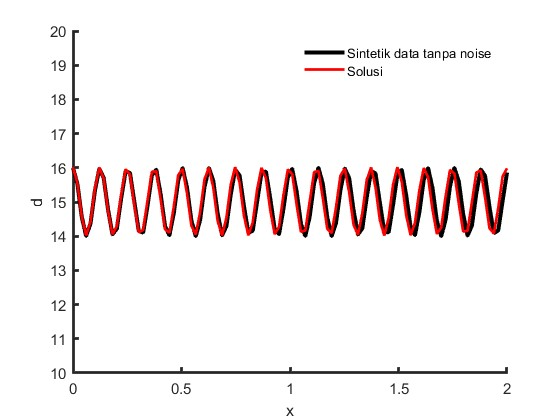
\includegraphics[width=10cm]{figure/gs true solution no noise.jpg}
    \caption{Grafik pencarian estimasi model dan model asli (true model) menggunakan metode Grid Search}
    \label{fig:gs true sol}
\end{figure}
\begin{figure}
    \centering
    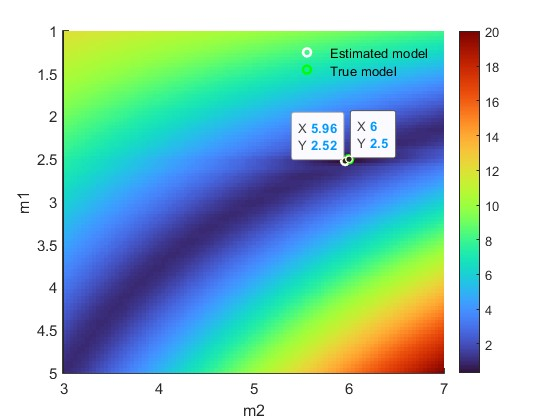
\includegraphics[width=10cm]{figure/gs true model no noise.jpg}
    \caption{Hasil pencarian model inversi $m_1$ dan $m_2$ menggunakan metode Grid Search}
    \label{fig:gs true mod}
\end{figure}


\subsection{Montecarlo Method}

Metode Montecarlo merupakan metode optimasi dengan menggunakan prinsip random search.
Di mana, pencarian solusi atau parameter model inversi dengan menggunakan optimasi Montecarlo ini dilakukan dengan cara tidak urut/tidak terstruktur seperti ketika dilakukan pencarian menggunakan optimasi Grid Search.
Pada metode Montecarlo, digunakan parameter tebakan inisial awal yang random.
Parameter tebakan awal random ini \textit{auto-generated} oleh syntax yang terdapat pada Matlab.
Tebakan awal, atau \textit{initial guess} akan di-\textit{generated} random dan parameter ini akan melakukan iterasi sampai iterasi maksimum di mana iterasi selanjutnya (iterasi setelah iterasi pertama sampai iterasi maksimum) juga akan dilakukan \textit{random} sampai parameter tebakan random ini menuju ke parameter model aslinya atau model awal yang ditentukan sebelumnya (mendekati $m_1$ dan $m_2$).

\begin{lstlisting}[caption={\textbf{montecarlo\textunderscore nonoise.m}}]
clc; clear all; close all;
% model awal acak dan fungsi objektifnya
N=200;
xmin=0;
xmax=2;
Dx=(xmax-xmin)/(N-1);
x = Dx*(0:N-1)';

% two model parameters
M=2;

% true model parameters
mt = [2.5, 6]';

% y=f(x, m1, m2);
w0=20;
dtrue = cos(w0*mt(1)*x) + mt(1)*mt(2);

L = 101;
Dm = 0.02;
m1min=1;
m2min=4.5;
m1a = m1min+Dm*(0:L-1)'; % m1a dari 0 2
m2a = m2min+Dm*(0:L-1)'; % m2a dari 0 2
m1max = m1a(L);
m2max = m2a(L);

% grid search, compute error, E
E = zeros(L,L);

for j = 1:L % kolom --> m1a
for k = 1:L % baris --> m2a
    dpre = cos(w0*m1a(j)*x) + m1a(j)*m2a(k); % perhitungan kedepan
    %no noise
    E(j,k) = sqrt((dtrue-dpre)'*(dtrue-dpre)/N); %RSME
    %with noise
    %E(j,k) = sqrt((dobs-dpre)'*(dobs-dpre)/N); %RSME

end
end

% plot data
figure(1);
clf;
set(gca,'LineWidth',2);
hold on;
axis( [m2min, m2max, m1min, m1max] );
axis ij;
imagesc([m2min, m2max], [m1min, m1max], E)
colormap("jet"); colorbar;

xlabel('m2');
ylabel('m1');
plot(mt(2), mt(1), 'go', 'LineWidth',2)

mg=[1,1]'; 
dg =cos(w0*mg(1)*x) + mg(1)*mg(2); 

%no noise
Eg =sqrt( (dtrue-dg)'*(dtrue-dg)/N);
%with noise
%Eg =sqrt( (dobs-dg)'*(dobs-dg)/N);

plot(mg(1),mg(2),'ko','LineWidth',3);

%xlabel('x');
%ylabel('d');
%%%%%%%%%


Niter=100;
Ehis=zeros(Niter+1,1);
m1his=zeros(Niter+1,1);
m2his=zeros(Niter+1,1);
Ehis(1)=Eg;
m1his(1)=mg(1);
m2his(2)=mg(2);

% randomly generate pairs of model parameters and check % if they further minimize the error 
ma=zeros(2,1); 
for k = 1:Niter

% randomly generate a solution 
ma(1) =random('unif',m1min,m1max); 
ma(2) =random('unif',m2min,m2max);

% compute its error 
da =cos(w0*ma(1)*x) + ma(1)*ma(2); 

%no noise
Ea=sqrt((dtrue-da)'*(dtrue-da)/N);
%with noise
%Ea=sqrt((dobs-da)'*(dobs-da)/N);

% adopt it if it is better 
if( Ea < Eg )

mg=ma;
Eg=Ea;
end

%save history
Ehis(1+k)=Eg;
m1his(1+k)=mg(1);
m2his(1+k)=mg(2);

h1=plot(mg(2), mg(1), 'wo', 'LineWidth',2);
plot([m2his(1+k-1), m2his(1+k)], [m1his(1+k-1), m1his(1+k)],'r','LineWidth',2)

end

%final model
m1est=m1his(Niter+1)
m2est=m2his(Niter+1)

h2=plot(mt(2),mt(1),'go','LineWidth',3);
legend([h1, h2],'Estimated model','True model');
legend boxoff ;
set(gca,'fontsize',11);
print(gcf,'Cluster','-djpeg','-r300');

figure(2);
clf;
subplot(3,1,1);
set(gca, 'FontSize', 11)
hold on;

plot(0:Niter, Ehis, 'k-', 'LineWidth',2);
xlabel('iteration');
ylabel('RMSE');
set(gca,'Fontsize',11);
subplot(3,1,2);
set(gca, 'LineWidth',2)
hold on;

plot([0,Niter], [mt(1), mt(1)], 'r', 'LineWidth',2);
plot(0:Niter, m1his, 'k-', 'LineWidth',2);
xlabel('iteration');
ylabel('m1');
set(gca, 'FontSize',11);
subplot(3,1,3);
set(gca, 'LineWidth',2)
hold on;

plot([0,Niter], [mt(2), mt(2)], 'r', 'LineWidth',2);
plot(0:Niter, m2his, 'k-', 'LineWidth',2);
xlabel('iteration');
ylabel('m2');
set(gca, 'FontSize',11);
print(gcf,'iterasi dan model-mc', '-djpeg', '-r300')
legend('True model','Estimated model');
hold on;

% evaluate prediction and plot it
figure(3)
clf;
set(gca,'LineWidth',2);
hold on;
axis( [0, xmax, 10, 20 ] );
%plot data

plot(x,dtrue, 'k-', 'LineWidth',2)
dpre = cos(w0*m1est*x) + m1est*m2est
plot(x,dpre,'r-','LineWidth',2);

xlabel('x');
ylabel('d');

%no noise
legend('Sintetik data tanpa noise','Solusi');

%with noise
%legend('Sintetik data tanpa noise','Sintetik data dengan noise','Solusi');

legend boxoff ;
set(gca,'fontsize',11);
print(gcf,'true and solution','-djpeg','-r300');

\end{lstlisting}

Dengan menggunakan \textit{code} di atas untuk pencarian solusi inverted model menggunakan metode montecarlo, maka didapatkan hasil pencarian sebagai berikut.
\begin{figure}[h]
    \centering
    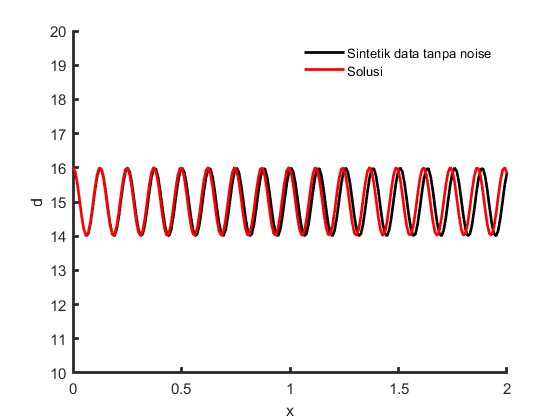
\includegraphics[width=10cm]{figure/mc true solution no noise.jpg}
    \caption{Grafik solusi estimasi model dan true model metode Montecarlo tanpa noise}
    \label{fig:mc true sol}
\end{figure}
\begin{figure}[h]
    \centering
    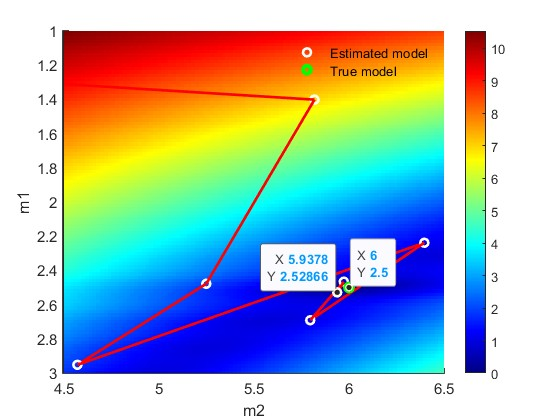
\includegraphics[width=10cm]{figure/mc true model no noise.jpg}
    \caption{Hasil \textit{true model} pencarian inversi metode Montecarlo tanpa noise}
    \label{fig:mc true model}
\end{figure}
\begin{figure}[h]
    \centering
    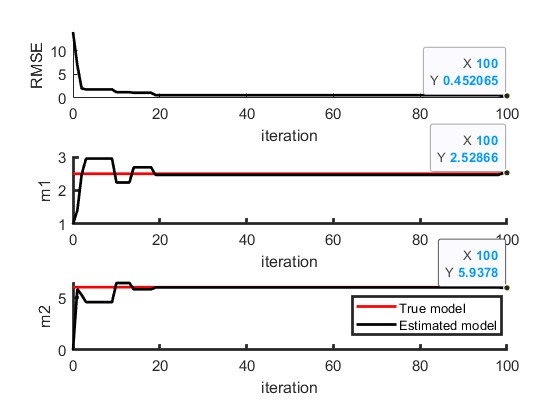
\includegraphics[width=10cm]{figure/mc rmse iterasi no noise.jpg}
    \caption{Hasil iterasi pencarian $m_1$ dan $m_2$ menggunakan metode optimasi Montecarlo tanpa noise}
    \label{fig:mc iterasi}
\end{figure}

\section{Jika $d_{obs}$ pada nomor 2 diberikan \textit{noise} dengan menggunakan \textit{random number} dari distribusi normal $\mu=0 \ ; \ \sigma=0.3$. \\
Tentukan Estimated Model $m_1$ dan $m_2$ menggunakan Grid Method dan Montecarlo Method}
\subsection{Grid Search Method with Noise}
Untuk mencari solusi \textit{inverted model} menggunakan metode Grid Search, digunakan cara yang sama seperti pada persoalan nomor 2, namun dengan penambahan \textit{noise} pada data \textit{true model}-nya. Kita dapat menggunakan \textit{code} di bawah ini (hanya menambahkan noise pada bagian $dtrue$).
\begin{lstlisting}[caption={\textbf{gridsearch\textunderscore addnoise}}]
% grid search with noise
clear all;close all;clc;

% data are in a simple auxillary variable, x
N=100;
xmin=0;
xmax=2.0;
Dx=(xmax-xmin)/(N-1);
x = Dx*(0:N-1)';

% two model parameters
M=2;

% true model parameters
mt = [2.5, 6.0]';

% y=f(x, m1, m2);
w0=20;
dtrue=cos(w0*mt(1)*x)+mt(1)*mt(2);

%with noise
sd=0.3;
dobs = dtrue + random('Normal',0,sd,N,1);

% plot data
figure(1);
clf;
set(gca,'LineWidth',2);
hold on;
axis( [0, xmax, 10, 20 ] );
plot(x,dtrue,'k-','LineWidth',3);

%with noise
plot(x,dobs,'bo-','LineWidth',1);

xlabel('x');
ylabel('d');


% 2D grid
L = 101;
Dm = 0.04;
m1min=1;
m2min=3;
m1a = m1min+Dm*(0:L-1)'; % m1a dari 0 2
m2a = m2min+Dm*(0:L-1)'; % m2a dari 0 2

m1max = m1a(L);
m2max = m2a(L);

% grid search, compute error, E
E = zeros(L,L);

for j = 1:L % kolom --> m1a
for k = 1:L % baris --> m2a
    dpre = cos(w0*m1a(j)*x) + m1a(j)*m2a(k); % perhitungan kedepan
    
    %no noise
    %E(j,k) = sqrt((dtrue-dpre)'*(dtrue-dpre)/N); %RSME

    %with noise
    E(j,k) = sqrt((dobs-dpre)'*(dobs-dpre)/N); %RSME
    

end
end

% find the minimum value of E and the corresponding (a b) value
[Erowmins, rowindices] = min(E);
[Emin, colindex] = min(Erowmins);
rowindex = rowindices(colindex);
m1est = m1min+Dm*(rowindex-1)
m2est = m2min+Dm*(colindex-1)

% evaluate prediction and plot it
dpre = cos(w0*m1est*x) + m1est*m2est
plot(x,dpre,'r-','LineWidth',2);

%no noise
%legend('Sintetik data tanpa noise','Solusi');

%with noise
legend('Sintetik data tanpa noise','Sintetik data dengan noise','Solusi');

legend boxoff ;
set(gca,'fontsize',11);
print(gcf,'true and solution grid search with noise','-djpeg','-r300');

figure(2);
clf;
set(gca,'LineWidth',2);
hold on;
axis( [m2min, m2max, m1min, m1max] );
axis ij;
imagesc( [m2min, m2max], [m1min, m1max], E);
colormap("turbo"); colorbar;
xlabel('m2');
ylabel('m1');
plot( m2est, m1est, 'wo', 'LineWidth', 2 );
plot( mt(2), mt(1), 'go', 'LineWidth', 2 );
    
legend boxoff ;
set(gca,'fontsize',11);
legend('Estimated model','True model');
print(gcf,'true-data gs with noise','-djpeg','-r300');

\end{lstlisting}

Dengan menggunakan source code \textbf{gridsearch\textunderscore addnoise} di atas, didapatkan grafik solusi yang ditunjukkan pada Gambar \ref{fig: gs noise sol} dan Gambar \ref{fig:gs noise truemod}.
\begin{figure}[h]
    \centering
    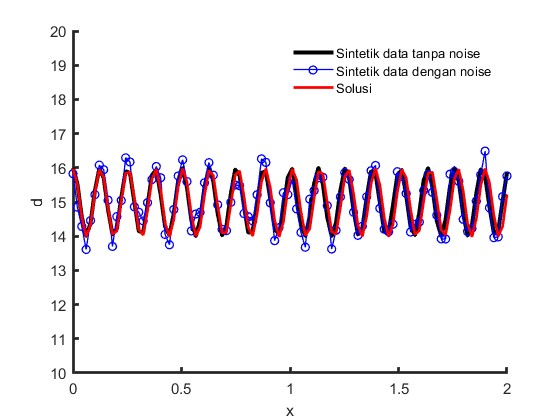
\includegraphics[width=10cm]{figure/gs noise true solution.jpg}
    \caption{Grafik solusi estimasi model dengan true model yang telah ditambahkan dengan noise menggunakan metode Grid Search}
    \label{fig: gs noise sol}
\end{figure}
\begin{figure}[h]
    \centering
    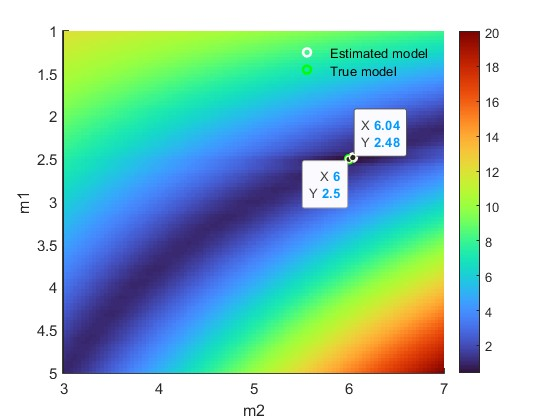
\includegraphics[width=10cm]{figure/gs noise true model.jpg}
    \caption{Solusi pencarian $m_1$ dan $m_2$ menggunakan metode Grid Search dengan true model yang telah ditambahkan noise}
    \label{fig:gs noise truemod}
\end{figure}


\subsection{Montecarlo Method with Noise}
Sama seperti bagian a namun berbeda metode saja, maka dapat digunakan source code \textbf{montecarlo\textunderscore add noise} di bawah ini untuk mencari solusi pendekatan $m_1$ dan $m_2$ menggunakan metode Montecarlo untuk data \textit{true model} yang telah ditambahkan noise.
Ingat bahwa noise ditambahkan pada bagian $dtrue$.
\begin{lstlisting}[caption={\textbf{montecarlo\textunderscore add noise}}]
clc; clear all; close all;
% model awal acak dan fungsi objektifnya
N=200;
xmin=0;
xmax=2;
Dx=(xmax-xmin)/(N-1);
x = Dx*(0:N-1)';

% two model parameters
M=2;

% true model parameters
mt = [2.5, 6]';

% y=f(x, m1, m2);
w0=20;
dtrue = cos(w0*mt(1)*x) + mt(1)*mt(2);

%with noise
sd=0.3;
dobs = dtrue + random('Normal',0,sd,N,1);

L = 101;
Dm = 0.02;
m1min=1;
m2min=4.5;
m1a = m1min+Dm*(0:L-1)'; % m1a dari 0 2
m2a = m2min+Dm*(0:L-1)'; % m2a dari 0 2
m1max = m1a(L);
m2max = m2a(L);

% grid search, compute error, E
E = zeros(L,L);

for j = 1:L % kolom --> m1a
for k = 1:L % baris --> m2a
    dpre = cos(w0*m1a(j)*x) + m1a(j)*m2a(k); % perhitungan kedepan
    %no noise
    %E(j,k) = sqrt((dtrue-dpre)'*(dtrue-dpre)/N); %RSME
    %with noise
    E(j,k) = sqrt((dobs-dpre)'*(dobs-dpre)/N); %RSME

end
end

% plot data
figure(1);
clf;
set(gca,'LineWidth',2);
hold on;
axis( [m2min, m2max, m1min, m1max] );
axis ij;
imagesc([m2min, m2max], [m1min, m1max], E)
colormap("jet"); colorbar;

xlabel('m2');
ylabel('m1');
plot(mt(2), mt(1), 'go', 'LineWidth',2)

mg=[1,1]'; 
dg =cos(w0*mg(1)*x) + mg(1)*mg(2); 

%no noise
%Eg =sqrt( (dtrue-dg)'*(dtrue-dg)/N);
%with noise
Eg =sqrt((dobs-dg)'*(dobs-dg)/N);

% plot data
plot(mg(1),mg(2),'ko','LineWidth',3);

%xlabel('x');
%ylabel('d');
%%%%%%%%%


Niter=100;
Ehis=zeros(Niter+1,1);
m1his=zeros(Niter+1,1);
m2his=zeros(Niter+1,1);
Ehis(1)=Eg;
m1his(1)=mg(1);
m2his(2)=mg(2);

% randomly generate pairs of model parameters and check % if they further minimize the error 
ma=zeros(2,1); 
for k = 1:Niter

% randomly generate a solution 
ma(1) =random('unif',m1min,m1max); 
ma(2) =random('unif',m2min,m2max);

% compute its error 
da =cos(w0*ma(1)*x) + ma(1)*ma(2); 

%no noise
%Ea=sqrt((dtrue-da)'*(dtrue-da)/N);
%with noise
Ea=sqrt((dobs-da)'*(dobs-da)/N);

% adopt it if it is better 
if( Ea < Eg )

mg=ma;
Eg=Ea; 
end

%save history
Ehis(1+k)=Eg;
m1his(1+k)=mg(1);
m2his(1+k)=mg(2);

h1=plot(mg(2), mg(1), 'wo', 'LineWidth',2);
plot([m2his(1+k-1), m2his(1+k)], [m1his(1+k-1), m1his(1+k)],'r','LineWidth',2)

end

%final model
m1est=m1his(Niter+1)
m2est=m2his(Niter+1)

h2=plot(mt(2),mt(1),'go','LineWidth',3);
legend([h1, h2],'Estimated model','True model');
legend boxoff ;
set(gca,'fontsize',11);
print(gcf,'Cluster with noise','-djpeg','-r300');

figure(2);
clf;
subplot(3,1,1);
set(gca, 'FontSize', 11)
hold on;

plot(0:Niter, Ehis, 'k-', 'LineWidth',2);
xlabel('iteration');
ylabel('RMSE');
set(gca,'Fontsize',11);
subplot(3,1,2);
set(gca, 'LineWidth',2)
hold on;

plot([0,Niter], [mt(1), mt(1)], 'r', 'LineWidth',2);
plot(0:Niter, m1his, 'k-', 'LineWidth',2);
xlabel('iteration');
ylabel('m1');
set(gca, 'FontSize',11);
subplot(3,1,3);
set(gca, 'LineWidth',2)
hold on;

plot([0,Niter], [mt(2), mt(2)], 'r', 'LineWidth',2);
plot(0:Niter, m2his, 'k-', 'LineWidth',2);
xlabel('iteration');
ylabel('m2');
set(gca, 'FontSize',11);
legend('True Model', 'Estimated Model')
print(gcf,'iterasi dan model-mc with noise', '-djpeg', '-r300')
hold on;

% evaluate prediction and plot it
figure(3)
clf;
set(gca,'LineWidth',2);
hold on;
axis( [0, xmax, 10, 20 ] );

%plot data
plot(x,dtrue, 'k-', 'LineWidth',2)
plot(x,dobs,'bo-','LineWidth',1)
dpre = cos(w0*m1est*x) + m1est*m2est
plot(x,dpre,'r-','LineWidth',2);

xlabel('x');
ylabel('d');

%with noise
legend('Sintetik data tanpa noise','Sintetik data dengan noise','Solusi');

legend boxoff ;
set(gca,'fontsize',11);
print(gcf,'true and solution with noise','-djpeg','-r300');
\end{lstlisting}
Setelah dilakukan \textit{running} pada \textit{code} di atas, didapatkan hasil pencarian model inversinya yang ditunjukkan pada Gambar \ref{fig: mc noise true sol}, \ref{fig: mc noise true mod}, dan \ref{fig: mc noise iterasi}.
\begin{figure}[h]
    \centering
    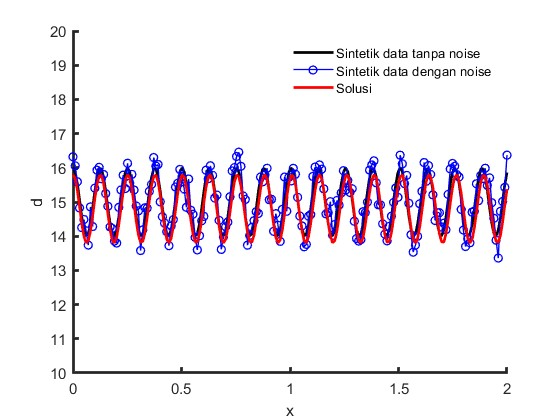
\includegraphics[width=10cm]{figure/mc noise true solution.jpg}
    \caption{Grafik estimasi pencarian $m_1$ dan $m_2$ menggunakan metode Montecarlo ketika $dtrue$ ditambahkan noise}
    \label{fig: mc noise true sol}
\end{figure}
\begin{figure}[h]
    \centering
    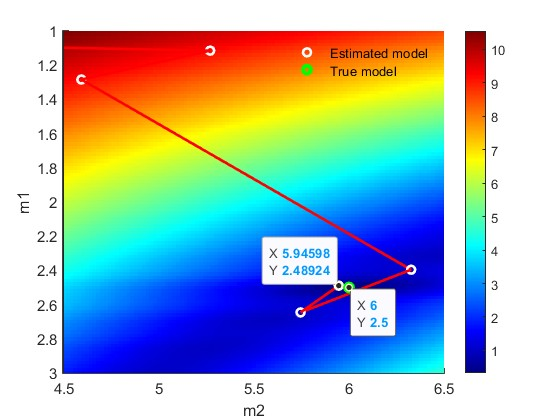
\includegraphics[width=10cm]{figure/mc noise true model.jpg}
    \caption{Hasil pencarian $m_1$ dan $m_2$ menggunakan metode Montecarlo ketika $dtrue$ ditambahkan noise}
    \label{fig: mc noise true mod}
\end{figure}
\begin{figure}[h]
    \centering
    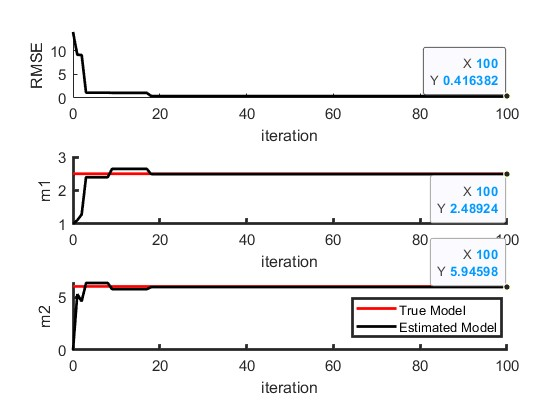
\includegraphics[width=10cm]{figure/mc noise rmse iterasi.jpg}
    \caption{Hasil iterasi pencarian $m_1$ dan $m_2$ ketika data asli ditambahkan noise dengan menggunakan pencarian metode optimasi Montecarlo}
    \label{fig: mc noise iterasi}
\end{figure}


\section{Apa pengaruh pemberian \textit{noise} pada persoalan nomor 3 jika dibandingkan dengan persoalan \textit{noise-free} yang terdapat pada soal nomor 2, terhadap hasil model inversi ($m_1$ dan $m_2$)?}

Noise yang diberikan pada data \textit{true model} berada pada rentang distribusi normal dengan standar deviasi $0.3$, di mana standar deviasi ini merupakan rentang nilai error yang berkisar antara $\pm 0.3$ yang diberikan secara acak kepada data \textit{true model}.
Sehingga, perbedaan solusi dari data awal sebelum dan sesudah dikenakan noise memiliki nilai yang tidak berbeda secara signifikan, namun tetap memiliki perbedaan solusi karena adanya faktor penambahan noise.
Setelah diberikan noise, dapat terlihat pada Gambar \ref{fig: gs noise sol} yang merupakan gambar hasil penambahan noise pada data asli, terdapat data yang tidak \textit{smooth} yang merupakan hasil dari penambahan noise. Data hasil penambahan noise ini yang menyebabkan nilai solusi pencarian estimasi $m_1$ dan $m_2$ yang berbeda dengan data awal tanpa dikenakan noise.
Perbedaan nilai solusi $m_1$ dan $m_2$ untuk metode Grid Search dapat dilihat perbandingannya pada Gambar \ref{fig:gs true mod} dengan Gambar \ref{fig:gs noise truemod}, dengan Gambar \ref{fig:gs noise truemod} merupakan solusi pencarian model menggunakan metode Grid Search ketika telah ditambahkan noise.
Sama seperti metode Grid Search, pada metode Montecarlo ketika data awal diberikan noise, juga terdapat perbedaan hasil solusi model 1 dan model 2, yang dapat dilihat pada Gambar \ref{fig:mc true model} untuk solusi sebelum dikenakan noise, dan pada Gambar \ref{fig: mc noise true mod} untuk pencarian model setelah dikenakan noise.
Dengan data penambahan noise pada data asli pencarian model pada metode Montecarlo setelah ditambahkan noise, dapat dilihat pada Gambar \ref{fig: mc noise true sol}.

Berikut ini merupakan tabel perbandingan data estimasi model sebelum dan setelah dikenakan noise.
\begin{table}[h!]
    \centering
    \caption{Perbandingan solusi model pada data sebelum dan sesudah dikenakan noise}
      \begin{tabular}{cccc}
        \toprule
        {Metode optimasi} & {\textit{true model} [$m_1$ $m_2$]} & \textit{estimated model} [$m_1$ $m_2$] & \textit{estimated model with noise} [$m_1$ $m_2$] \\
   \midrule
      Grid Search & [$2.5$ \ $6.0$] & [$2.52$ \ $5.96$] & [$2.48$ \ $6.04$] \\
      Montecarlo & [$2.5$ \ $6.0$] & [$2.5287$ \ $5.9378$] & [$2.4892$ \ $5.9460$]\\
      \bottomrule
      \end{tabular}%
    \label{tab:bentuk geometri}%
\end{table}%



\end{document}